\documentclass[../main.tex]{subfiles}

\begin{document}
\begin{questions}

\question Consider a thin spherical shell (thickness $\to$ 0) of radius $R$ with a surface charge density
\begin{equation*}
	\sigma(\theta) = \sigma_0(\cos\theta + \cos^2\theta)
\end{equation*}
Using solutions of Laplace's equation, find the potential $V (r,\theta)$ everywhere, both for $r > R$ and $r < R$.

\begin{solution}
	As before, we know that,
	\begin{align}
		V_\text{out}(r,\theta) &= \sum_{l=0}^{\infty} \frac{B_l}{r^{l+1}}P_l(\cos\theta)\\
		V_\text{in}(r,\theta) &= \sum_{l=0}^{\infty} A_lr^lP_l(\cos\theta)
	\end{align}
	We can apply $V_\text{in}(R,\theta) = V_\text{out}(R,\theta)$ to get $B_l = A_l R^{2l+1}$\\
	We also know that
	\begin{align}
		\sigma(\theta) &= \epsilon_0 \left.\frac{\partial V_\text{in}(r,\theta)}{\partial r}\right|_{r=R} - \epsilon_0\left.\frac{\partial V_\text{out}(r,\theta)}{\partial r}\right|_{r=R}\\
		&= \epsilon_0\sum_{l=0}^{\infty} (2l+1) A_l R^{l-1} P_l(\cos\theta)
		\intertext{We can immediately see that $A_l = 0$ $\forall$ $l>2$. Comparing coefficients,}
		\sigma_0\cos\theta + \sigma_0\cos^2\theta &= \frac{A_0\epsilon_0}{R} + 3A_1\epsilon_0\cos\theta + \frac{5A_2R\epsilon_0}{2}\left(3\cos^2\theta - 1\right)\\
		\implies A_2 &= \frac{2\sigma_0}{15R\epsilon_0}\\
		A_1 &= \frac{\sigma_0}{3\epsilon_0}\\
		A_0 &= \frac{\sigma_0R}{3\epsilon_0}
	\end{align}
	Thus we can write the potentials
	\begin{align}
		V_\text{out} &= \frac{\sigma_0R^2}{3\epsilon_0r} + \frac{\sigma_0R^3}{3\epsilon_0r^2}\cos\theta + \frac{\sigma_0R^4}{15\epsilon_0r^3}\left(3\cos^2\theta -1\right)\\
		V_\text{in} &= \frac{\sigma_0R}{3\epsilon_0} + \frac{\sigma_0r}{3\epsilon_0}\cos\theta + \frac{\sigma_0r^2}{15\epsilon_0R}\left(3\cos^2\theta -1\right)
	\end{align}
\end{solution}

\question In the following system (see figure), the inner conducting sphere of radius $a$ carries charge $Q$ and the outer sphere of radius $b$ is grounded. The distance between the centres is $c$ which is a small quantity.
\begin{center}
	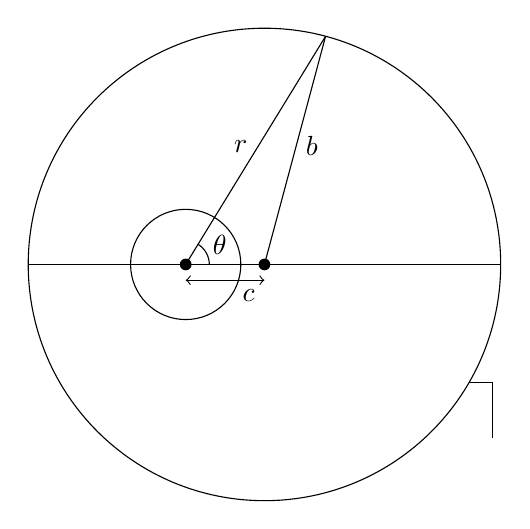
\begin{tikzpicture}
		\draw (0,0) circle (0.7);
		\draw (1,0) circle (3);

		\draw (0,0) -- ({1+3*cos(75)},{3*sin(75)});
		\draw (1,0) -- ({1+3*cos(75)},{3*sin(75)});

		\draw (-2,0) -- (4,0);

		\node at (0,0)[circle,fill,inner sep=1.5pt]{};
		\node at (1,0)[circle,fill,inner sep=1.5pt]{};

		\draw[<->] (0,-0.2) -- (1,-0.2) node[below left]{$c$};
		\node at (0.7,1.5){$r$};
		\node at (1.6,1.5){$b$};

		\draw (0.3,0) arc (0:58.4:0.3);
		\node at ({0.5*cos(30)}, {0.5*sin(30)}){$\theta$};

		\draw ({1+3*cos(30)}, {-3*sin(30)}) -- ({1.3+3*cos(30)}, {-3*sin(30)}) -- ({1.3+3*cos(30)}, {-0.7-3*sin(30)}) node{$\Ground$};
	\end{tikzpicture}

\end{center}

\begin{parts}
	\part Show that to the first order in $c$, the equation describing the outer sphere, using the centre of inner sphere as origin, is $r(\theta)=b+c\cos\theta$.
	\begin{solution}
		We can use trigonometry and observe
		\begin{align}
			b^2 &= c^2 + r^2 - 2cr\cos\theta
			\intertext{Solving using the Quadratic Formula (and taking the positive root)}
			r &= c\cos\theta + \sqrt{b^2-c^2\sin^2\theta}\\
			&= c\cos\theta + b\sqrt{1-\frac{c^2\sin^2\theta}{b^2}}\\
			&= c\cos\theta + b\left(1-\frac{c^2\sin^2\theta}{2b^2}\right) + \mathcal{O}(c^4)\\
			&= b + c\cos\theta + \mathcal{O}(c^2)
		\end{align}

		We can also see this geometrically
		\begin{center}
			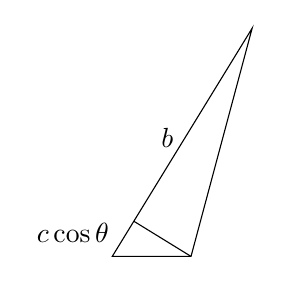
\begin{tikzpicture}
				\draw (0,0) -- ({1+3*cos(75)},{3*sin(75)}) -- (1,0) -- cycle;
				\draw (1,0) -- ({cos(58.4)^2},{cos(58.4)*sin(58.4)});

				\node at (-0.5,0.3){$c\cos\theta$};
				\node at (0.7,1.5){$b$};
			\end{tikzpicture}
		\end{center}
	\end{solution}

	\part If the potential between two spheres contains only $l = 0$ and $l = 1$ angular components, determine it to first order in $c$.
	\begin{solution}
		As before, we have
		\begin{align}
			V(r,\theta) &= \sum_{l=0}^{\infty} \left(A_l r^l + \frac{B_l}{r^{l+1}}\right)P_l(\cos\theta)
		\end{align}
		\begin{align}
			\frac{\partial V(a,\theta)}{\partial \theta} &= 0 && \text{Inner sphere equipotential} \label{eq:7bc1}\\
			-\epsilon_0 \int_{\text{inner sphere}}\left.\frac{\partial V(r,\theta)}{\partial r}\right|_{r=a} &= Q && \text{Total charge on inner sphere} \label{eq:7bc2}\\
			V(b+c\cos\theta+\mathcal{O}(c^2),\theta) &= 0 && \text{Outer sphere grounded}\label{eq:7bc3}
		\end{align}
		Using \eqref{eq:7bc1},
		\begin{align}
			B_l = -A_l a^{2l+1} \,\forall\,l > 0
		\end{align}
		Using, \eqref{eq:7bc2}
		\begin{align}
			-2\pi\epsilon_0a^2 \int_{\theta=0}^{\pi} \left(-\frac{B_0}{a^2} +\sum_{l=1} (2l+1)A_la^{l-1}P_l(\cos\theta)\right)\sin\theta\,d\theta = Q\\
			\implies 4\pi\epsilon_0B_0 + \sum_{l=1}^{\infty} a^{l+1} (2l+1) A_l \int_{x=-1}^{1} P_l(x)\,dx=Q\\
			\implies 4\pi\epsilon_0B_0 + \sum_{l=1}^{\infty} a^{l+1} (2l+1) A_l \int_{x=-1}^{1} P_l(x)P_0(x)\,dx=Q\\
			\implies B_0 = \frac{Q}{4\pi\epsilon_0}
		\end{align}
		Applying \eqref{eq:7bc3}
		\begin{align}
			0 &= A_0 + B_0\left(b + c\cos\theta + \mathcal{O}(c^2)\right)^{-1} \\
			&+ \left(A_1\left(b + c\cos\theta + \mathcal{O}(c^2)\right)+B_1\left(b + c\cos\theta + \mathcal{O}(c^2)\right)^{-2}\right)\cos\theta + \mathcal{O}(\cos^2\theta)
		\end{align}
		\begin{align}
			\implies A_0 + \frac{B_0}{b} + \left(A_1b + \frac{B_1}{b^2}-\frac{B_0c}{b^2}\right)\cos\theta + \mathcal{O}(c^2) + \mathcal{O}(\cos^2\theta) = 0
		\end{align}
		Solving upto first order in $c$ and equating coefficients of $1$ and $\cos\theta$,
		\begin{align}
			A_0 &= -\frac{Q}{4\pi\epsilon_0b}\\
			A_1 &= -\frac{Q}{4\pi\epsilon_0(b^3-a^3)}
		\end{align}
		Putting it all together,
		\begin{align}
			V(r,\theta) &= \frac{Q}{4\pi\epsilon_0}\left(\frac{1}{r}-\frac{1}{b}-\frac{c}{b^3-a^3}\left(r-\frac{a^3}{r^2}\right)\cos\theta\right) + \mathcal{O}(c^2) + \mathcal{O}(\cos^2\theta)
		\end{align}
	\end{solution}
\end{parts}

\question Static charges are distributed along the $x$ axis (one-dimensional) in the interval $-a \leq x' \leq a$. The
charge density is :
\begin{equation*}
	\begin{cases}
		\rho(x') & -a \leq x' \leq a\\
		0 & |x'| > a 
	\end{cases}
\end{equation*}

\begin{parts}
	\part Write down the multipole expansion for the electrostatic potential $\phi(x)$ at a point $x$ on the axis in terms of $\rho(x')$, valid for $x > a$
	\begin{solution}
		\begin{align}
			\phi(x) &= \frac{1}{4\pi\epsilon_0}\int_{x=-a}^{a} \frac{\rho(x')}{|x-x'|}dx'\\
			\phi(x) &= \frac{1}{4\pi\epsilon_0}\int_{x=-a}^{a} \frac{\rho(x')}{x|1-\frac{x'}{x}|}dx'\\
			&= \frac{1}{4\pi\epsilon_0}\int_{x=-a}^{a} \frac{\rho(x')}{x}\,dx' + \frac{1}{4\pi\epsilon_0}\int_{x=-a}^{a} \frac{\rho(x')x'}{x^2}\,dx' + \frac{1}{4\pi\epsilon_0}\int_{x=-a}^{a} \frac{\rho(x')x'^2}{x^3}\,dx'\dots\\
			&= \sum_{l=0}^{\infty} \frac{1}{4\pi\epsilon_0} \int_{x=-a}^{a} \frac{\rho(x')x'^{l}}{x^{l+1}}\,dx' 
		\end{align}
	\end{solution}

	\part For each charge configuration given in below figure, find (a) total charge $Q=\int \rho(x')\,dx'$, (b) dipole moment $P =\int x'\rho(x')\,dx'$
	\begin{center}
		(I)
		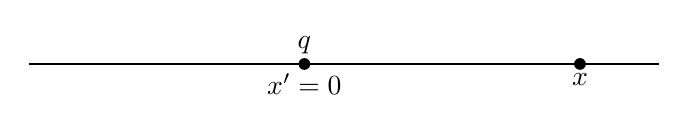
\begin{tikzpicture}
			\draw[thick] (-4,0) -- (4,0);
			\node at (-0.5,0)[circle,fill,inner sep=1.5pt]{};
			\node at (3,0)[circle,fill,inner sep=1.5pt]{};

			\node at (-0.5,0)[above]{$q$};
			\node at (-0.5,0)[below]{$x'=0$};

			\node at (3,0)[below]{$x$};
		\end{tikzpicture}\\
		(II)
		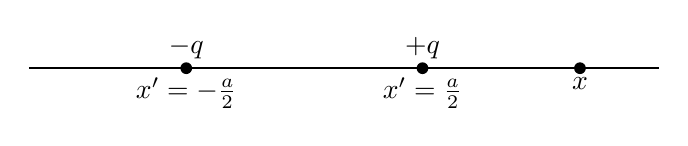
\begin{tikzpicture}
			\draw[thick] (-4,0) -- (4,0);
			\node at (-2,0)[circle,fill,inner sep=1.5pt]{};
			\node at (1,0)[circle,fill,inner sep=1.5pt]{};
			\node at (3,0)[circle,fill,inner sep=1.5pt]{};

			\node at (-2,0)[above]{$-q$};
			\node at (-2,0)[below]{$x'=-\frac{a}{2}$};

			\node at (1,0)[above]{$+q$};
			\node at (1,0)[below]{$x'=\frac{a}{2}$};

			\node at (3,0)[below]{$x$};
		\end{tikzpicture}\\
		(III)
		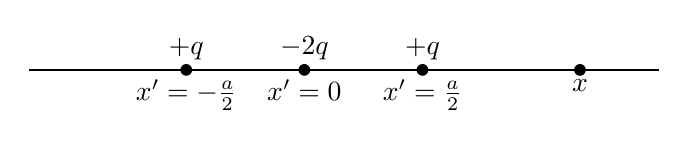
\begin{tikzpicture}
			\draw[thick] (-4,0) -- (4,0);
			\node at (-2,0)[circle,fill,inner sep=1.5pt]{};
			\node at (1,0)[circle,fill,inner sep=1.5pt]{};
			\node at (-0.5,0)[circle,fill,inner sep=1.5pt]{};
			\node at (3,0)[circle,fill,inner sep=1.5pt]{};

			\node at (-2,0)[above]{$+q$};
			\node at (-2,0)[below]{$x'=-\frac{a}{2}$};

			\node at (-0.5,0)[above]{$-2q$};
			\node at (-0.5,0)[below]{$x'=0$};

			\node at (1,0)[above]{$+q$};
			\node at (1,0)[below]{$x'=\frac{a}{2}$};

			\node at (3,0)[below]{$x$};
		\end{tikzpicture}
	\end{center}

	\begin{solution}
		(I) $Q = q$, $P = 0$\\
		(II) $Q = 0$, $P = qa$\\
		(III) $Q = 0$, $P = 0$ 
	\end{solution}
\end{parts}

\question A circular disc of radius $R$ lies in the $z = 0$ plane, centred at the origin. It has the following charge density frozen on
\begin{equation*}
	\sigma(r',\phi) = \sigma_0 r'\cos(\phi)
\end{equation*}
\begin{parts}
	\part What is the monopole moment of the configuration?
	\begin{solution}
		\begin{align}
			Q &= \int_{\text{all space}} \rho\,d\tau\\
			&= \sigma_0\int_{r'=0}^{R}\int_{\phi=0}^{2\pi} r'^2\cos\phi\,dr'\,d\phi\\
			&= 0
		\end{align}
	\end{solution}

	\part Calculate the dipole contribution to the potential due to the configuration at $(0, 0, z)$ using the expression in polar form
	\begin{solution}
		We know that $\theta' = \frac{\pi}{2}$, so $\cos\theta' = 0$, therefore dipole contribution is also $0$
	\end{solution}

	\part Now calculate the the cartesian components of the dipole moment of the conguration. Use this to calculate the dipole contribution at $(0, 0, z)$. Verify your answer with the expression obtained in (b)
	\begin{solution}
		\begin{align}
			\vec{P} &= \int_{\text{disc}} \vec{r}\rho(r')\,d\tau'\\
			&= \sigma_0\int_{r'=0}^{R}\int_{\phi=0}^{2\pi} r'^3(\cos\phi\,\ihat + \sin\phi\,\jhat)\cos\phi\,dr'\,d\phi\\
			&= \frac{\pi\sigma_0R^4}{4}\,\ihat
		\end{align}

		$V(0,0,z) = \frac{1}{4\pi\epsilon_0 z^2} \frac{\pi\sigma_0R^4}{4}\,\ihat \cdot \khat = 0$
	\end{solution}
\end{parts}

\question If the total amount of charge (monopole) contained in a distribution is zero, show that the dipole moment is independent of the choice of the origin.

\begin{solution}
	\begin{align}
		\vec{P} &= \int \vec{r'}\rho(\vec{r'})\,d\tau'\\
		\intertext{$\vec{r'}\to\vec{r'}-\vec{a}$}
		\vec{P}_1 &= \int \vec{r'}\rho(\vec{r'})\,d\tau' - \vec{a}\int \rho(\vec{r'})\,d\tau'\\
		&= \int \vec{r'}\rho(\vec{r'})\,d\tau' = \vec{P}
	\end{align}
\end{solution}

\question Find the dipole moment of:
\begin{parts}
	\part A ring with charge per unit length $\lambda = \lambda_0\cos\phi$ where $\phi$ is the angular variable in cylindrical coordinates.
	\begin{solution}
		\begin{align}
			\vec{P} &= \lambda_0 R^2\int_{\phi=0}^{2\pi} (\cos\phi\,\ihat + \sin\phi\,\jhat)\cos\phi\,d\phi\\
			&= \lambda_0 \pi R^2 \,\ihat
		\end{align}
	\end{solution}

	\part A sphere with charge per unit area $\sigma = \sigma_0 \cos \theta$ where $\theta$ is the polar angle measured from the positive $z$ axis.
	\begin{solution}
		\begin{align}
			\vec{P} &= \sigma_0R^3 \int_{\theta=0}^{\pi}\int_{\phi=0}^{2\pi} (\sin\theta\cos\phi\,\ihat + \sin\theta\sin\phi\,\jhat + \cos\theta\khat) \cos\theta\sin\theta\,d\theta\,d\phi\\
			&= \frac{4\pi}{3} \sigma_0 R^3\,\khat
		\end{align}
	\end{solution}
\end{parts}

\question An electric dipole of moment $\vec{P} = (P_x, 0, 0)$ is located at the point $(x_0, y_0, 0)$ where $x_0 > 0$ and $y_0 > 0$. The planes $x = 0$ and $y = 0$ are conducting plates with a tiny gap at the origin. The potential of the plate at $x = 0$ is maintained at $V_0$ and the plate at $y = 0$ is grounded. The dipole is sufficiently weak so that you can ignore the charges induced on the plates.
\begin{center}
	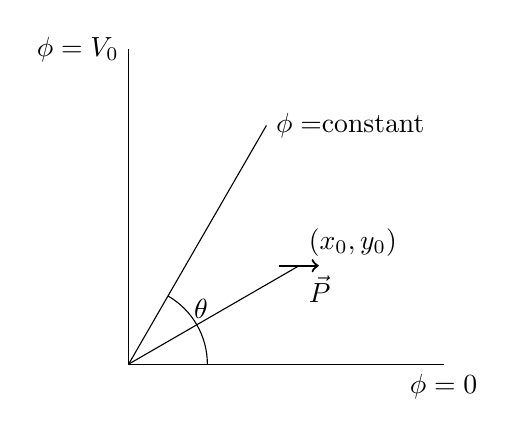
\begin{tikzpicture}
		\draw (0,4) node[left]{$\phi=V_0$} -- (0,0) -- (4,0) node[below]{$\phi=0$};

		\draw (0,0) -- ({2.5*cos(30)},{2.5*sin(30)}) node[above right]{$(x_0, y_0)$} node[below right]{$\vec{P}$};
		\draw[thick,->] ({-0.25 + 2.5*cos(30)},{2.5*sin(30)}) -- ({0.25 + 2.5*cos(30)},{2.5*sin(30)});

		\draw (0,0) -- ({3.5*cos(60)},{3.5*sin(60)}) node[right]{$\phi=$constant};
		\draw (1,0) arc (0:60:1);
		\node at ({cos(45)},{sin(45)})[right]{$\theta$};
	\end{tikzpicture}
\end{center}
\begin{parts}
	\part Based on the figure, deduce a simple expression for the electrostatic potential $\phi(x, y)$.
	\begin{solution}
		We need to solve the equations
		\begin{align}
			\frac{1}{\rho}\frac{\partial}{\partial \rho}\rho\frac{\partial \phi(\rho,\theta)}{\partial \rho}+\frac{1}{\rho^2}\frac{\partial^2 \phi(\theta)}{\partial \theta^2} = 0 && \text{Laplace's Equation}\\
			\phi(\rho,0) = 0 && \text{Boundary Conditions}\label{eq:cbc1}\\
			\phi(\rho,\frac{\pi}{2}) = V_0\label{eq:cbc2}
		\end{align}
		in the region $0 \leq \theta \leq \frac{\pi}{2}$\\
		We can write the general solution using separation of variables (the linear solution in $\theta$ no longer needs to be periodic since our domain is no longer the full range of $\theta$)
		\begin{align}
			\phi(\rho,\theta) &= (A_0+B_0\ln\rho)(C_0 + D_0\theta) + \sum_{m=1}^{\infty}(A_m\rho^m + B_m\rho^{-m})(C_m\cos m\theta + D_m \sin m\theta)
		\end{align}
		Applying \eqref{eq:cbc1} and \eqref{eq:cbc2}
		\begin{align}
			B_0 &= 0\\
			C_m &= 0\, \forall \,m\\
			D_m &= 0\, \forall \,m > 0\\
		\end{align}
		We are left with
		\begin{align}
			\phi(\rho,\theta) &= A_0D_0\theta
		\end{align}
		Applying \eqref{eq:cbc2} gives us $A_0D_0 = \frac{2V_0}{\pi}$
		\begin{align}
			\implies \phi(\theta) &= \frac{2V_0}{\pi}\theta\\
			\implies \phi(x,y) &= \frac{2V_0}{\pi}\tan^{-1}\left(\frac{y}{x}\right)
		\end{align}
	\end{solution}

	\part Calculate the force on the dipole
	\begin{solution}
		\begin{align}
			\vec{E} &= -\nabla \phi\\
			&= -\frac{1}{\rho} \frac{2V_0}{\pi}\,\hat{\theta}\\
			&= \frac{2V_0y}{\left(x^2+y^2\right)\pi}\,\ihat - \frac{2V_0x}{\left(x^2+y^2\right)\pi}\,\jhat\\
			\vec{F} &= (\vec{P}\cdot\nabla)\vec{E}\\
			&= -\frac{4V_0x_0y_0P_x}{\left(x_0^2+y_0^2\right)^2\pi}\,\ihat + \left(-\frac{2V_0P_x}{(x_0^2+y_0^2)\pi}+\frac{4V_0x_0^2P_x}{(x_0^2+y_0^2)^2\pi}\right)\,\jhat\\
			&= \frac{2V_0P_x}{(x_0^2+y_0^2)^2\pi}\left(2x_0y_0\,\ihat + (x_0^2-y_0^2)\,\jhat\right)
		\end{align}
	\end{solution}
\end{parts}

\end{questions}
\end{document}